Caching policies, controlled through HTTP headers, significantly impact page load times by reducing the need for repeated 
resource requests. Effective caching policies leverage client-side (browser caching) and intermediate server storage 
(proxy caching). \\
\\
\textbf{Proxy caching} involves storing copies of web resources at intermediate proxy servers, which can then serve subsequent requests 
for the same resources without contacting the origin server. This reduces network latency and bandwidth usage.\\
\\
\textbf{Browser caching} involves storing web resources locally on the client's device, allowing subsequent page visits to be loaded 
faster without the need to re-download the same resources.\\
\\
\textbf{Implementation}: the implementation of caching policies is facilitated through the use of the 'Cache-Control' header in HTTP responses. 
This header allows servers to communicate specific caching directives to clients and intermediaries. It provides instructions such as the maximum 
time a resource should be considered fresh ('max-age') and whether the resource can be cached by intermediate proxies ('public') or the browser ('private').
To ensure the validity of cached resources, several headers are utilized in caching strategies. The 'Expires' header specifies the date and time after which 
the resource should be considered stale. The 'Last-Modified' header indicates the date and time of the resource's last modification. Additionally, 
the 'Etag' header provides a unique identifier for the resource. These headers enable three main non-mutually exclusive strategies for validating 
cached resources: 'Expiration', 'Validation', and 'Heuristic'. The \textbf{Expiration} and \textbf{Heuristic} strategies generally result in faster response times, 
as they rely on pre-determined expiration dates or heuristics to determine the freshness of the cached resources. On the other hand, 
the \textbf{Validation} strategy requires a round-trip to the server to confirm the validity of the cached resources, resulting in slower response times.

\subsubsection{Caching mechanisms}
To evaluate the impact of caching policies on page load times, various websites with different caching strategies leveraging the browser cache were tested. 
The results, as depicted in Figure \ref{fig:2_site_policy}, clearly demonstrate the benefits of caching. Enabling caching led to a significant reduction 
in page load times across all tested websites. 

    \begin{figure}[H]
        \centering
        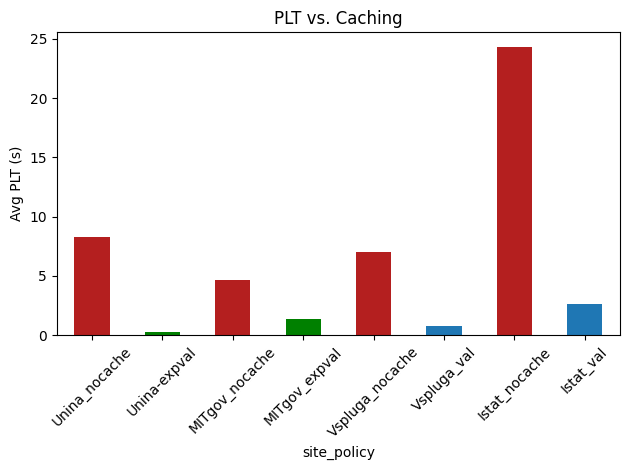
\includegraphics[width=0.48\textwidth]{2_site_policy.png}
        \caption{\small Caching policies of the tested websites}
        \label{fig:2_site_policy}
    \end{figure}

Interestingly, when comparing the specific methods used to validate cached resources (validation and exp+validation), no noticeable differences were observed (Figure \ref{fig:2_policy}).
This observation can be attributed to two factors. Firstly, websites can implement different caching policies for various resources, making it challenging 
to discern distinct impacts on page load times. Secondly, the performance gap between the 'Expiration' and 'Validation' strategies primarily arises 
when the resources are cached and not yet expired, allowing the 'Expiration' strategy to be leveraged. However, verifying this fact requires a thorough 
examination of individual resources, which is not easily feasible.

    \begin{figure}[H]
        \centering
        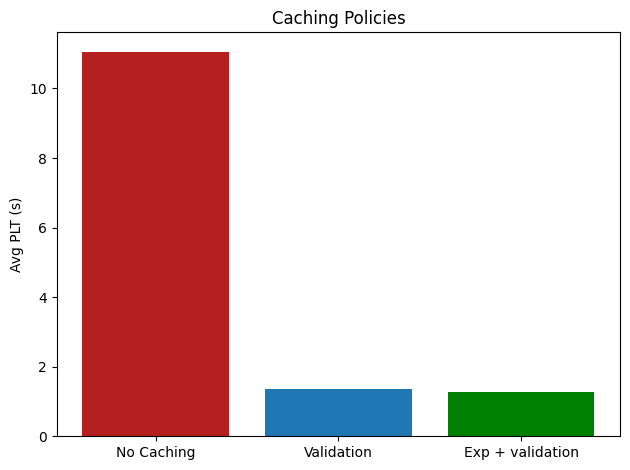
\includegraphics[width=0.48\textwidth]{2_policy.png}
        \caption{\small Page Load Time (PLT) vs. Caching Policy}
        \label{fig:2_policy}
    \end{figure}

In conclusion, even though the 'Expiration', 'Validation', and 'Heuristic' strategies have their advantages and trade-offs, the overall performance 
benefits of caching are evident.

\subsubsection{Caching and HTTP version}
Over the years, multiple versions of the HTTP protocol have been released, each introducing new features and improvements. 
HTTP/1.1 brought advancements such as persistent connections, pipelining, and caching. These enhancements aimed to enhance the efficiency 
of resource delivery. Building on this foundation, HTTP/2 introduced significant improvements, including binary framing, multiplexing, server push, 
and header compression. These features further optimized the protocol's performance.
HTTP/3, the latest version, introduced a new transport protocol called QUIC, which is based on UDP (User Datagram Protocol), as opposed to 
the previous versions that relied on TCP (Transmission Control Protocol). This change in the underlying transport protocol offers potential benefits such as 
improved latency, better congestion control, and enhanced security.
Despite these protocol advancements, the fundamental caching system remains unchanged and relies on headers.
To practically assess the performance impact of different HTTP versions and the influence of caching, a website (Off-White) was subjected to 
testing. The website was tested using different versions of the HTTP protocol, with caching enabled and disabled. The experimental results are depicted 
in Figure \ref{fig:3_version_caching}.

    \begin{figure}[H]
        \centering
        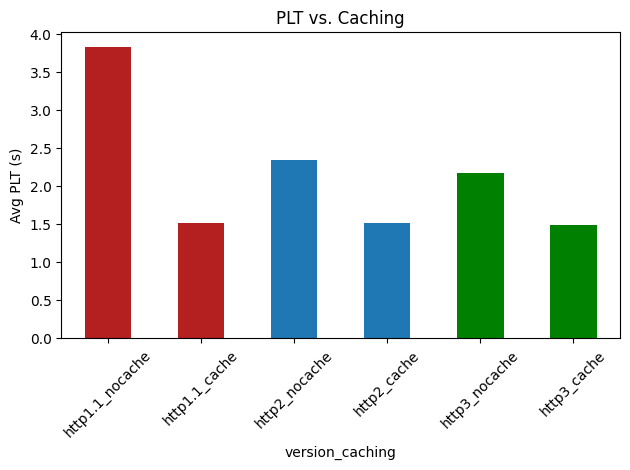
\includegraphics[width=0.48\textwidth]{3_version_caching.png}
        \caption{\small Page Load Time (PLT) vs. HTTP version and caching}
        \label{fig:3_version_caching}
    \end{figure}

As anticipated, enabling caching resulted in a substantial decrease in page load times for all tested versions of the HTTP protocol. 
The uniformity of loading times with caching enabled suggests that the caching mechanism played a more prominent role in influencing performance than the 
specific protocol version being used. This underscores the significance of efficient caching strategies in optimizing overall page load times.\\
Another interesting observation is depicted in Figure \ref{fig:3_version}. As expected, each new protocol version outperforms the previous one.
This performance improvement is not dependent on caching mechanism and it is attributable to the above discussed enhancements brought by each new version.

    \begin{figure}[H]
        \centering
        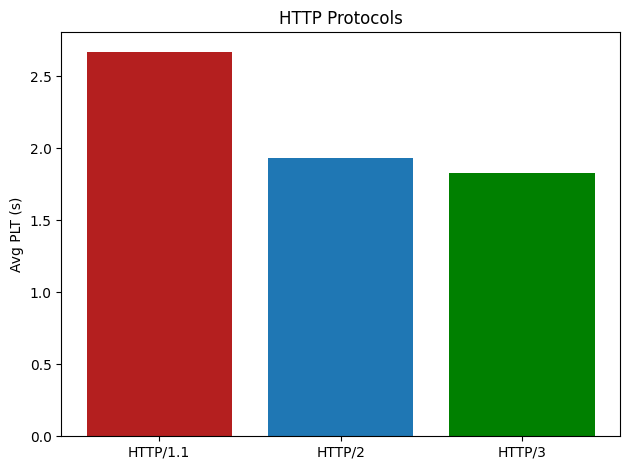
\includegraphics[width=0.48\textwidth]{3_version.png}
        \caption{\small Page Load Time (PLT) vs. HTTP version}
        \label{fig:3_version}
    \end{figure}
